\documentclass[10pt,letter]{article}

\usepackage{amsmath}
\usepackage{url}
\usepackage{amssymb}
% packages that allow mathematical formatting

\usepackage{graphicx}
% package that allows you to include graphics

\usepackage{setspace}
% package that allows you to change spacing

\usepackage{cite}
% for BibTeX

\usepackage{algpseudocode}
\usepackage{algorithmicx}
\usepackage{algorithm}

\usepackage[sc,osf]{mathpazo}
\linespread{1.05}         % Palatino needs more leading
\usepackage[T1]{fontenc}

\fontencoding{T1}
\fontfamily{ppl}
\fontseries{m}
\fontshape{n}
\fontsize{10}{13}
% Set font size. The first parameter is the font size to switch to; the second
% is the \baselineskip to use. The unit of both parameters defaults to pt. A
% rule of thumb is that the baselineskip should be 1.2 times the font size.
\selectfont

\usepackage{parskip}
% Use the style of having no indentation with a space between paragraphs.

\usepackage{enumitem}
% Resume an enumerated list, continuing the old numbering, after some
% intervening text.

% \usepackage{fullpage}
% package that specifies normal margins

\usepackage{titling}
% move the title up a bit, wastes less space
\setlength{\droptitle}{-5em}

\usepackage{caption}
\usepackage{subcaption}
% for subfigures

\usepackage[usenames,dvipsnames]{color}
% for \color used in listings
\usepackage{textcomp}
% for upquote used in listings
\usepackage{listings}
\lstset{
    breakatwhitespace, % somehow prevents lstinline from line splitting
    tabsize=2,
    rulecolor=,
    basicstyle=\footnotesize,
    upquote=true,
    aboveskip={1.5\baselineskip},
    columns=fixed,
    extendedchars=true,
    breaklines=true,
    prebreak = \raisebox{0ex}[0ex][0ex]{\ensuremath{\hookleftarrow}},
    frame=single,
    showtabs=false,
    showspaces=false,
    showstringspaces=false,
    keywordstyle=\color{Purple},
    identifierstyle=\color{Black},
    commentstyle=\color{BrickRed},
    stringstyle=\color{RubineRed},
    captionpos=b,
}
\lstloadlanguages{erlang}
\lstset{language=erlang}

\usepackage{tikz}
\usetikzlibrary{backgrounds}
\usetikzlibrary{fit}
\usetikzlibrary{positioning}
\usetikzlibrary{shapes.misc} % for cross shaped nodes

\pgfdeclarelayer{b}
\pgfdeclarelayer{f}
\pgfsetlayers{b,main,f}

\newcommand{\plate}[4]{
\begin{pgfonlayer}{b}
\node (invis#1) [draw, color=white, inner sep=1pt,rectangle,fit=#2] {};
\end{pgfonlayer}
\begin{pgfonlayer}{f}
\node (capt#1) [ below left=0 pt of invis#1.south east, xshift=2pt,yshift=1pt, fill=black!15]
{\footnotesize{#3}};
\end{pgfonlayer}
\begin{pgfonlayer}{b}
\node (#1) [fill=black!15, rounded corners, inner sep=5pt, rectangle,fit=(invis#1) (capt#1),#4] {};
\end{pgfonlayer}
}

%%%%%%%%%%%%%%%%%%%%%%%%%%%%%%%%%%%%%%%%%%%%%%%%%%%%%%%%%%%%%%%%%%%%%%%%%%%%%%%
%% Macros

\newcommand{\chubby}[0]{\textsc{Chubby}}
\newcommand{\phat}[0]{\textsc{Phat}}
\newcommand{\phatraid}[0]{\textsc{PhatRaid}}
\newcommand{\phatraidcf}[2]{\textsc{PhatRaid}(#1,#2)}
\newcommand{\raid}[1]{\textsc{RAID #1}}
\newcommand{\paxos}[0]{\textsc{Paxos}}
%%%%%%%%%%%%%%%%%%%%%%%%%%%%%%%%%%%%%%%%%%%%%%%%%%%%%%%%%%%%%%%%%%%%%%%%%%%%%%%

\begin{document}

\title{PHAT RAID, yo}
\author{Andrew Johnson \and Daniel King \and Lucas Waye \and Scott Moore}
\date{May 13, 2014}

\maketitle

Distributed file stores, like Google's \chubby{} and CS260r's \phat{}, send all
files through a single master node which consistently replicates the file on
many slaves. In this scheme, the master node's throughput is a bottleneck for
storing large files. We present \phatraid{} which mitigates this bottleneck by
partitioning files across many \paxos{} groups which form a \raid{1} group.

\section{Introduction}

\subsection{Disk Performance}

An important consideration in our project is the impact disk performance has on overall commit latency. We believe that disk read/write latency is the major contributor to storing large files in a distributed system. {\bf TODO more}

In a review of hard disk performance \cite{disk-perf}, Hard Disk Drives (HDD) were compared with Solid State Drives (SSD). HDDs use a physical magnetic platter that spins so that a drive head can read or write data by sensing or manipulating the magnetic field in a particular position on to the platter. In contrast, SSDs have no moving parts and instead uses integrated circuits as memory to store data persistently. Because the way in which data is accessed is different, the performance characteristics between the two are different.

\begin{figure}
\centering
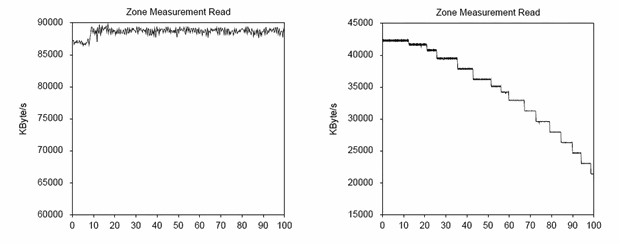
\includegraphics[width=\textwidth]{disk-perf}
\caption{{\bf Left Chart}: Solid State Disk reads across entire drive (Left -- Outermost sector, Right -- Innermost sector), {\bf Right Chart}: Hard Disk reads across the entire drive (Left -- Outer rim, Right -- Inner rim). From \cite{disk-perf}}
\label{fig:hdd-vs-sdd}
\end{figure}

Figure \ref{fig:hdd-vs-sdd} shows a comparison between read times for a SSD and HDD as a function of position on the disk. HDD storage performance is greatly influenced by where on the disk platter the data was placed. Data can be placed on the outer rim of the platter much more quickly than data placed near the center of the platter as the outer rim is moving faster in comparison (due to conservation of angular momentum). In contrast to HDDs, SSDs do not exhibit this problem as there is no spinning platter. The right diagram in \ref{fig:hdd-vs-sdd} shows relatively constant read performance throughout the entire disk. Additionally, HDDs have difficultly with random accesses as the drive may need to wait for the drive head to be directly over the correct position on the platter. This problem becomes especially apparent when an individual file is fragmented into multiple blocks by the file system. SSDs have relatively better random access times, in general, than HDDs. Sequential access tends to be many times faster than random access for both SSDs and HDDs \cite{disk-perf}. HDD performance can also can suffer from {\em spin-up delay}, which happens as a result of a power-saving measure that stops spinning the disk during idle times.

We decided that HDDs have far too much performance variability in order to be properly modeled. As a result, we instead chose to simulate the performance characteristics of SSDs as they have relatively constant access times regardless of sector position on the drive and also do not suffer from {\em spin-up delay}.

\urldef\hwbenchmark\url{http://www.tomshardware.com/charts/ssd-charts-2013/benchmarks%2C129.html}
\begin{figure}
\centering
\begin{tabular}{l || c}
\multicolumn{2}{c}{{\bf Solid State Disk Performance Benchmarks}} \\ \hline
Sequential Write Speed  \hspace{7em} & 55.03 - 481.85 MB/sec \\ 
Write Access Time & 0.03 - 0.32 ms \\ \hline
Sequential Read Speed &  207.95 - 522.45 MB/sec \\
Read Access Time & 0.03 - 0.22 ms \\ \hline
\end{tabular}
\caption[Solid State Performance]{Solid State Disk performance for middle 95\% of solid state drives tested in a benchmark. Benchmark available at Benchmark available at \hwbenchmark.}
\label{fig:sdd-perf}
\end{figure}

Figure \ref{fig:sdd-perf} shows the performance for SSDs from a 2013 survey of commercially available SSDs. Sequential write speeds measure the throughput (in megabytes per second) of data stored on the drive when the data is being written in the drive's natural sequential order (e.g. increasing sectors). Similarly, sequential read speed measures the throughput for sequential reads. Read/Write access times represent the latency of performing a single random read or write. 

\section{Implementation}

\subsection{Erlang Primer}

\phatraid{} is implemented in Erlang. Erlang is a pure, functional language with
extensive library support for distributed applications. Erlang has one unit of
concurrency, the process, and one unit of distribution, the node. Each Erlang
node consists of an arbitrary number of processes. Erlang nodes may live on the
same machine or on different machines connected by a network. Every Erlang node
is given a name by an Erlang name server. Erlang processes may communicate with
any Erlang node which they can name. Erlang processes interact with one another
by making RPC calls.

\subsection{System Organization}

\begin{figure}
  \centering
  \begin{tikzpicture}
    [<->,scale=.85,shorten <=2pt, shorten >=2pt,]
    \node [rectangle, draw, thick, inner sep=5pt] (raidclient) at (0,2) {Raid Client};
    \node [rectangle, draw, thick, inner sep=5pt] (client1) at (-4,1) {Client 1};
    \node [rectangle, draw, thick, inner sep=5pt] (client2) at (0,0) {Client 2};
    \node [rectangle, draw, thick, inner sep=5pt] (client3) at (4,1) {Client 3};
    \node [rectangle, draw, thick, inner sep=5pt] (vr11) at (-6, -2) {Replica};
    \node [rectangle, draw, thick, inner sep=5pt] (vr12) at (-4, -2) {Master};
    \node [rectangle, draw, thick, inner sep=5pt] (vr13) at (-2, -2) {Replica};
    \node [rectangle, draw, thick, inner sep=5pt] (vr21) at (-2, -4) {Replica};
    \node [rectangle, draw, thick, inner sep=5pt] (vr22) at (0, -4) {Master};
    \node [rectangle, draw, thick, inner sep=5pt] (vr23) at (2, -4) {Replica};
    \node [rectangle, draw, thick, inner sep=5pt] (vr31) at (2, -2) {Replica};
    \node [rectangle, draw, thick, inner sep=5pt] (vr32) at (4, -2) {Master};
    \node [rectangle, draw, thick, inner sep=5pt] (vr33) at (6, -2) {Replica};


    \foreach \to in {client1, client2, client3}
      \draw [thick] (raidclient) -- (\to);
    \draw [thick] (client1) -- (vr12);
    \draw [thick] (client2) -- (vr22);
    \draw [thick] (client3) -- (vr32);

    % \foreach \to in {vr11, vr13}
    %   \draw [thick] (vr12) -- (\to);
    % \foreach \to in {vr21, vr23}
    %   \draw [thick] (vr22) -- (\to);
    % \foreach \to in {vr31, vr33}
    %   \draw [thick] (vr32) -- (\to);

    \plate{clientnode}{(raidclient)(client1)(client2)(client3)}{Client Node}{}
    \plate{pc1}{(vr11)(vr12)(vr13)}{Phat Cluster \#1}{}
    \plate{pc2}{(vr21)(vr22)(vr23)}{Phat Cluster \#2}{}
    \plate{pc3}{(vr31)(vr32)(vr33)}{Phat Cluster \#3}{}

  \end{tikzpicture}
  \caption{A \phatraidcf{3}{1} Group}
  \label{fig:organization}
\end{figure}

\phatraid{} is implemented in Erlang, reusing our previous implementation of
\phat{}. The implementation is divided into three domains: the server cluster,
the client, and the raid-client. The server code implements a VR-like consensus
algorithm as well as simple file system. The client code exposes a file system
API which hides the communication bookkeeping. The raid-client provides a file
system API which transparently partitions files and reassembles them as they are
sent and received from the server cluster.

Figure \ref{fig:organization} depicts the organization of our system. The
raid-client delegates communication to each client. Each client is connected to
one \phat{} cluster, which has a master and a number of replicas.

Each \phat{} cluster maintains a file system which is separate and distinct from
the file systems of other \phat{} clusters. Generally, two phat clusters do not
communicate.

\subsection{Disk Emulation and Abstraction Layer}

We developed a novel ``{\bf {\em Disk Emulation and Abstraction Layer}}'' (DEAL)
to simulate SSD performance so they .

\subsection{RAIDing \phat{}}

A \phatraidcf{$C$}{$f$} implementation is parameterized by two numbers: $C$, the
number of \phat{} clusters, and $f$, the \phat{} cluster failure threshold. A
single \phat{} cluster contains $2f + 1$ nodes. A \phatraid{} group contains $C$
clusters for a total of $C(2f+1)$ \phat{} nodes. A \phatraid{} group can be
concurrently accessed by an arbitrary number of raid-clients.

On a client node, the raid-client spawns $C$ client processes which each maintain
a connection to one of the $C$ \phat{} clusters. All communications between the
raid-client and a phat cluster go through the assigned client process.

\subsection{Erlang Behaviors}

In Erlang, the basic unit of concurrency is a \emph{process} and an Erlang VM is
known as a \emph{node}. A process may communicate with other processes on its
node as well as processes on other nodes. Multiple nodes may be on the same
machine or distributed across many machines.

The server cluster is implemented as a collection of nodes running the same
server code. One of these nodes is designated the master node. The other nodes
are known as replicas.

The master and each replica has four components: the supervisor, the
(unfortunately named) server, VR, and the file system.

\begin{itemize}
\item the supervisor -- if any of the other three processes dies, it shuts all
  of them down and restarts all of them
\item the server -- if the node is the master, it passes messages on to VR; if
  the node is a replica, it redirects clients to the master
\item VR -- maintains a log of opaque messages, achieving consensus with other
  nodes in the cluster via the Viewstamped Replication protocol
\item the file system -- a simple hierarchical file system with locks
\end{itemize}

The four components are implemented using Erlang behaviors. An Erlang behavior
is a framework which implements common patterns like servers and finite state
machines. In particular, the supervisor uses the \texttt{supervisor} behavior,
the server and file system both use the \texttt{gen\_server} behavior, and VR
uses the \texttt{gen\_fsm} behavior.

\begin{itemize}
\item The \texttt{supervisor} behavior provides a framework for restarting
  failed processes.
\item The \texttt{gen\_server} behavior provides a framework for many-client
  single-server interactions. We implemented functions to process messages
  formatted as Erlang tuples. The \texttt{gen\_server} behavior handles
  low-level socket interaction.
\item The \texttt{gen\_fsm} behavior generalizes the \texttt{gen\_server}
  behavior by permitting the server to have a finite number of states. Each
  state has a set of functions with which to process messages. This behavior can
  be seen as an ad hoc polymorphic variant of the \texttt{gen\_server} behavior.
\end{itemize}

Additionally, the \texttt{gen\_server} and \texttt{gen\_fsm} behaviors allow
the programmer to specify an arbitrary state value which will be passed around
\`{a} la functional reactive programming.

\subsubsection{The \texttt{supervisor} Behavior}

\lstinputlisting[firstline=6,lastline=18,float,
                 caption=The \texttt{supervisor} Behavior --- \texttt{phat.erl},
                 label=lst:supervisor,
                 numbers=left, firstnumber=6]
                {../phat.erl}

Listing \ref{lst:supervisor} is taken from our supervisor code. When a
supervisor is started, the \texttt{supervisor} behavior looks for a unary
procedure called \lstinline!init!. The \lstinline!init! procedure returns a
child specification which is a pair of a restart specification and a list of
children. In Listing \ref{lst:supervisor}, the restart specification,
\lstinline!{one_for_all,1,5}! specifies that if any one node dies, all nodes
should be restarted, unless more than one failure has occurred in the past five
seconds. If more than one failure occurs in five seconds, the supervisor kills
all the children and shuts itself down as well.

Each child in the list of children is a 6-tuple consisting of: child name,
initial procedure call, child transience, shutdown style, child type, necessary
modules.

\begin{itemize}
\item The initial procedure call is a 3-tuple of module, procedure name and
  argument list.
\item Every child's transience is specified as \lstinline!permanent!, meaning
  they should be restarted.
\item Every child has shutdown style \lstinline!1! meaning they will first be
  asked to terminate and one second later they will be forcibly terminated.
\item All of our children are workers, which are distinguished from
  sub-supervisors.
\item The necessary modules are dynamically loaded when the child processes is
  initialized, there is a one-to-one mapping between our children and code
  modules.
\end{itemize}

\subsubsection{The \texttt{gen\_fsm} Behavior}

\begin{lstlisting}[float,caption=The \texttt{gen\_fsm} Behavior --- \texttt{vr.erl},
                   label=lst:genfsm, numbers=left, firstnumber=176]
replica( {prepare, MasterViewNumber, _, _, _, _, _}
       , State = #{ viewNumber := ViewNumber})
    when MasterViewNumber > ViewNumber ->
    ?debugFmt("my view is out of date, need to recover~n", []),
    startRecovery(State);

replica( {prepare, MasterViewNumber, _, _, _, _, _}
       , State = #{ timeout := Timeout, viewNumber := ViewNumber})
    when MasterViewNumber < ViewNumber ->
    ?debugFmt("ignoring prepare from old view~n", []),
    {next_state, replica, State, Timeout};

replica( { prepare, _, Op, OpNumber
         , MasterCommitNumber, Client, RequestNum}
       , State = #{ prepareBuffer := PrepareBuffer }) ->
    Message = {OpNumber, Op, Client, RequestNum},
    NewPrepareBuffer = lists:sort([Message|PrepareBuffer]),
    processPrepareOrCommit( OpNumber
                          , MasterCommitNumber
                          , NewPrepareBuffer
                          , State
                          );
\end{lstlisting}

\begin{lstlisting}[float,caption={Processing the VR Message Queue, Part 1 --- \texttt{vr.erl}},
                   label=lst:processing1, numbers=left, firstnumber=375]
processPrepareOrCommit( OpNumber, MasterCommitNumber, NewPrepareBuffer
                      , State = #{ timeout := Timeout
                                 , commitNumber := CommitNumber
                                 , masterNode := MasterNode
                                 , myNode := MyNode
                                 , viewNumber := ViewNumber
                                 , allNodes := Nodes})
  when CommitNumber > MasterCommitNumber ->
    NewViewNumber = ViewNumber + 1,
    NewMaster = chooseMaster(State, NewViewNumber),
    sendToReplicas( MasterNode
                  , Nodes
                  , {startViewChange, NewViewNumber, MyNode}
                  ),
    { next_state
    , viewChange
    , State#{ viewNumber := NewViewNumbern
            , masterNode := NewMaster }
    , Timeout
    };
\end{lstlisting}
\begin{lstlisting}[float,caption={Processing the VR Message Queue, Part 2 --- \texttt{vr.erl}},
                   label=lst:processing2, numbers=left, firstnumber=397]
processPrepareOrCommit( OpNumber, MasterCommitNumber, NewPrepareBuffer
                      , #{ timeout := Timeout } = State) ->
    AfterBuffer =
      processBuffer( State#{ prepareBuffer := NewPrepareBuffer }
                   , NewPrepareBuffer
                   , MasterCommitNumber
                   ),
    AfterLog = processLog(AfterBuffer, MasterCommitNumber),
    #{ masterNode := MasterNode
     , viewNumber := ViewNumber
     , commitNumber := CommitNumber
     , myNode := MyNode } = AfterLog,
    if
        CommitNumber < MasterCommitNumber ->
            startRecovery(State);
        true ->
            sendToMaster( MasterNode
                        , {prepareOk, ViewNumber, OpNumber, MyNode}
                        ),
            {next_state, replica, AfterLog, Timeout}
    end.
\end{lstlisting}

A state in the \texttt{gen\_fsm} behavior manifests as a procedure which accepts
two arguments: the incoming message and the store\footnote{Mutable state is
  implemented as a pure store value which is passed around by the behavior}. The
return value of a state-procedure is usually the 4-tuple
\lstinline!{next_state,NextState,NewStore,Timeout}!. The \texttt{gen\_fsm}
behavior will transition to \lstinline!NextState! and set the store to
\lstinline!NewStore!. When a new message is received the \texttt{gen\_fsm}
behavior will invoke the \lstinline!NextState! procedure with the new message
and the \lstinline!NewStore!.

We implemented Viewstamped Replication\cite{liskov2012viewstamped} to achieve
consensus in the file system. Listing \ref{lst:genfsm} defines how to handle
prepare messages sent to a node in the replica state. It is piecewise defined by
pattern matching on the arguments. The first two definition clauses use the
\lstinline!when! keyword to specify arbitrary required relationships between the
matched variables.

The final definition clause triggers when the replica receives a message in the
current view. The replica adds the message to a sorted queue and calls a
processing procedure. The processing procedure is defined separately in Listing
\ref{lst:processing1} and Listing \ref{lst:processing2}.

Listing \ref{lst:processing1} handles a message from an out-of-date master,
i.e., his commit number is older than the replica's commit number. The replica
first proposes a view change to the cluster. Afterwards, it changes its
\texttt{gen\_fsm} state to \lstinline!viewChange! and updates the
store\footnote{The store is called \lstinline!State! in the code listings} with
the new view number and the new master.

Listing \ref{lst:processing2} handles messages from the current master. The
\lstinline!prepareBuffer! stores prepare messages that arrived out of order. In
particular, if the log ends at operation number $n$ and message $n+1$ is dropped
by the network, all subsequent messages will be buffered. The buffered messages
will not be added to the log until message $n+1$ is received. The call to
\lstinline!processBuffer! moves messages to the log, if all previous messages
have now been received. The call to \lstinline!processLog! commits new messages
in the log which have been committed by the master node. Lines 405 to 408
destructure \lstinline!AfterLog! and bind variables for later use. The final
\lstinline!if! statement responds to the master unless the master has committed
messages we haven't received.\footnote{This can happen if the network drops a message whose
  operation number lies between the replica's last commit number and the
  master's last commit number.}

\section{Evaluation}

\subsection{Resilience}

We distinguish between two types of failure: cessation of progress and loss of
data. In a VR cluster without persistent stores, data loss only occurs when all
$2f+1$ nodes in the cluster fail. In a VR cluster, progress only ceases if $f+1$
nodes are lost. In \phatraid{} the conditions for cessation of progress and loss
of data are complicated by the combination of RAID and VR.

\begin{figure}
  \centering
  \begin{subfigure}{0.4\textwidth}
    \centering
    \begin{tikzpicture}[<->,scale=.5,shorten <=2pt, shorten >=2pt,]
      \foreach \x/\y in {1/1, 1/2, 1/3, 2/1, 2/2, 2/3, 3/1, 3/2, 3/3}
        \node [circle, draw, thick] (pr\x\y) at (\x,-\y) {};
      \foreach \x/\y in {3/1, 3/2, 3/3, 1/3, 2/3}
        \node [strike out, draw=red, thick] (pr\x\y) at (\x,-\y) {};
    \end{tikzpicture}
    \caption{Progress, No Data Loss}
    \label{fig:failures_allok}
  \end{subfigure}
~
  \begin{subfigure}{0.4\textwidth}
    \centering
    \begin{tikzpicture}[<->,scale=.5,shorten <=2pt, shorten >=2pt,]
      \foreach \x/\y in {1/1, 1/2, 1/3, 2/1, 2/2, 2/3, 3/1, 3/2, 3/3}
        \node [circle, draw, thick] (pr\x\y) at (\x,-\y) {};
      \foreach \x/\y in {1/1, 1/2, 2/1, 2/2}
        \node [strike out, draw=red, thick] (pr\x\y) at (\x,-\y) {};
    \end{tikzpicture}
    \caption{No Progress, No Data Loss}
    \label{fig:failures_noprogress}
  \end{subfigure}
\\\vspace{1em}
  \begin{subfigure}{0.4\textwidth}
    \centering
    \begin{tikzpicture}[scale=.5,shorten <=2pt, shorten >=2pt,]
      \node[rotate=25] (N) at (1.5,-1.5) {\textsc{Impossible!}};
    \end{tikzpicture}
    \caption{Progress, Data Loss}
    \label{fig:failures_max}
  \end{subfigure}
~
  \begin{subfigure}{0.4\textwidth}
    \centering
    \begin{tikzpicture}[<->,scale=.5,shorten <=2pt, shorten >=2pt,]
      \foreach \x/\y in {1/1, 1/2, 1/3, 2/1, 2/2, 2/3, 3/1, 3/2, 3/3}
        \node [circle, draw, thick] (pr\x\y) at (\x,-\y) {};
      \foreach \x/\y in {1/1, 1/2, 1/3, 2/1, 2/2, 2/3}
        \node [strike out, draw=red, thick] (pr\x\y) at (\x,-\y) {};
    \end{tikzpicture}
    \caption{No Progress, Data Loss}
    \label{fig:failures_noprogress_nodata}
  \end{subfigure}

  \caption{Some Failed Node Distributions of \phatraidcf{3}{1}}
  \label{fig:failures}
\end{figure}

Four distributions of failed nodes in \phatraidcf{3}{1} are depicted in Figure
\ref{fig:failures}. In this section, if we claim ``data is lost'', we mean that
if no persistent store is used, data will be lost. Adding a persistent store
obviously prevents loss of committed data.

The top left corner depicts five of the nine nodes failing. This state is
\emph{not} a failure state. The group can still make progress and no data is
lost. The two surviving clusters can reach consensus on new values and can
reconstruct the failed cluster's data.

The top right corner depicts four of the nine nodes failing. This state is a
failure state. The group cannot make progress but no data can been
lost. Progress is blocked because more than one cluster cannot reach
consensus. Since no cluster was completely destroyed, all data still exists on
at least one node.

The bottom left corner is impossible because if data can be lost then we
certainly cannot make progress.

The bottom right corner depicts six of the nine nodes failing. This state is
also a failure state. The group cannot make progress and will lose
data. Progress is blocked because more than one cluster cannot reach
consensus. Additionally, two complete clusters have been lost so half of the
data cannot be recovered.

In general, progress ceases if more than one cluster cannot reach consensus and
data loss occurs if more than one cluster completely fails. The lower bound of
failed nodes for progress cessation in \phatraidcf{$C$}{$f$} is:
    $$ C\cdot(f+1) $$
and the lower bound of failed nodes for data loss is:
    $$ 2\cdot(2f+1) $$

In contrast, if all data has been propagated to all nodes, data is only lost
when all nodes die. If data has not been propagated to all nodes, then loss
occurs if all nodes containing the data die. 

\subsection{Performance}

\section{Conclusion}

\bibliographystyle{plain}
\bibliography{paper}

\end{document}
